\documentclass{beamer}
\usepackage[utf8]{inputenc}
\usepackage{graphicx}
\usepackage{url}

\author[Sowmya Vajjala]{Instructor: Sowmya Vajjala}


\title[LING 120]{LING 120: \\ Language and Computers}
\subtitle{Semester: Fall '17}

\date{03 November 2017}

\institute{Iowa State University, USA}

%%%%%%%%%%%%%%%%%%%%%%%%%%%

\begin{document}

\begin{frame}\titlepage
\end{frame}

\begin{frame}
\frametitle{Outline for today}
\begin{itemize}
\item Discussion about Wednesday's question
\item Dialog Systems - conclusion
\item Assignment 6 Description
\item Overview of speech recognition
\item Next week: Speech processing continued
\item Reminder: Assignment 5 due tomorrow!!
\end{itemize}	
\end{frame}

\begin{frame}
\frametitle{Wednesday's Exercise}
The Yes Bot: \url{http://www.nacloweb.org/resources/problems/2013/N2013-L.pdf}
\begin{itemize}
\item Give an example of a sentence that, when said by the CEO, will cause Yesbot to make a mistake.
\item Provide two examples of words that, when the CEO uses them in a sentence, will sometimes cause
Yesbot to make a mistake, but sometimes won’t. Explain why.
\item Are there any words that will always cause Yesbot to make a mistake, (that is, say a lie) any time the
CEO uses them? List any you can, and explain why or why not.
\end{itemize}
\end{frame}

\begin{frame}
\frametitle{Your Responses-1}
\begin{itemize}
\item Question 1: Give an example of a sentence that, when said by the CEO, will cause Yesbot to make a mistake.
\item Response 1: "I have a lot of power." "Yes, sir or ma'am, it is true that I have a lot of power."
\item Response 2: "I can't believe Dave thought he would get my job!" "Yes, sir or ma'am, it is true that I can't believe Dave thought he would get my job." Obviously, the owner can believe it, so the statement that Yesbot replies with is false.
\end{itemize}
\end{frame}

\begin{frame}
\frametitle{Your Responses-2}
\begin{itemize}
\item Question 2: Provide two examples of words that, when the CEO uses them in a sentence, will sometimes cause
Yesbot to make a mistake, but sometimes won’t. Explain why.
\item Response 1: "I" because a sentence that is strictly about the CEO wont make sense, but if the CEO says "I" and "you" in the same       sentence then it can make sense. "Yes, sir or ma'am, it is true that I know the secrets", "Yes, sir or ma'am, it is true that you and I know the secrets"
\end{itemize}
\end{frame}

\begin{frame}
\frametitle{Your Responses-3}
\begin{itemize}
\item Question 3: Are there any words that will always cause Yesbot to make a mistake, (that is, say a lie) any time the
CEO uses them? List any you can, and explain why or why not. 
\item Response 1: "Any type of homophone could make yesbot mess up. The program might be confused and use the wrong word or wrong form of a word. (ex. new and knew)"
\item Other Responses: Words I and You, First and second person pronouns, question words, terms indicating commands. 
\item Answer from the solution: \url{http://www.nacloweb.org/resources/problems/2013/N2013-LS.pdf}
\end{itemize}
\end{frame}

\begin{frame}
\frametitle{Dialog Systems - Quick summary}
We discussed:
\begin{itemize}
\item What are dialog systems, where are they useful? 
\item What are the different kinds of dialog systems? How are they built?
\item How can we evaluate dialog systems?
\item What are some dialog systems that are used in current day world?
\end{itemize}
\end{frame}

\begin{frame}
\frametitle{If you found this interesting ..}
\begin{itemize}
\item Dialog systems are a very fascinating, and active area of research and development.
\item Lot of scope for interesting jobs and projects, lot of cool work to do! \pause
\item To get a hang of what the real "dialog systems" people do (not in a 100 level course!), you can check out the following:
\begin{itemize}
\item Speech and Language Processing textbook by Jurafsky and Martin (draft chapters online 29--30 are about Dialog systems: \url{https://web.stanford.edu/~jurafsky/slp3/})
\item A course on Spoken Dialog system taught at UW: \url{http://courses.washington.edu/ling575/SPR2017/index.html} 
\item Some readings from a Deep Learning course at UPenn: \url{http://dialog-systems-class.org/readings.html}
\end{itemize} \pause
\item If you know how to program, start writing your own version of Eliza or Parry! 
\end{itemize}
\end{frame}

\begin{frame}
\frametitle{Assignment 6 Description}
\begin{itemize}
\item Theme: Descriptive writeups about dialog systems, addressing specific questions.
\item 10\% of your grade
\item Due on 18th November
\item Details on Canvas
\end{itemize}
%http://nacloweb.org/resources/problems/2009/N2009-F.pdf
\end{frame}

\begin{frame}
\frametitle{About Final Exam}
\begin{itemize}
\item Final Exam is 20\% of your grade
\item It is a 3-step process of which one step is done in class - if you miss that class, you don't get grade for that.
\item You don't have sit in an exam center in the exams week!
\item All details on Canvas, but I will more on this in the week before thanksgiving break!
\item I will try to update topics by Monday though, so that you have enough time to think.
\end{itemize}
\end{frame}

\begin{frame}
\frametitle{}
\Large Our next topic: Speech processing
\end{frame}

\begin{frame}
\frametitle{Questions to get you started -1}
\begin{itemize}
 \item How should we make a computer understand Speech? \pause
\item According to you, what are the steps involved in speech recognition? \pause
\item When a computer sees text, it breaks it down character by character, each character has some Unicode rep and so on. How does that work with Speech? \pause
\item If we map sounds (instead of characters) to a new alphabet (phonetic alphabet), that will make all sounds converted to alphabet - will it fix the problem? \pause
\item What do you think are difficult to make out with this kind of mapping - vowel sounds or consonant sounds? \pause
\item Once we map alphabet to sounds successfully, what else is left over? 
\end{itemize}
\end{frame}

\begin{frame}
\frametitle{Representing Pronunciation Symbolically, as Transcribed text}
\begin{itemize}
\item The International Phonetic Alphabet (IPA) is an evolving standard whose goal is to transcribe the sounds of all human languages in a uniform manner. 
\\ (\url{https://en.wikipedia.org/wiki/International_Phonetic_Alphabet})
\item Something specific to American English: ARPABet
\\ \url{https://en.wikipedia.org/wiki/ARPABET}
\end{itemize}
\end{frame}

\begin{frame}
\frametitle{Phonetic Transcription - Example}
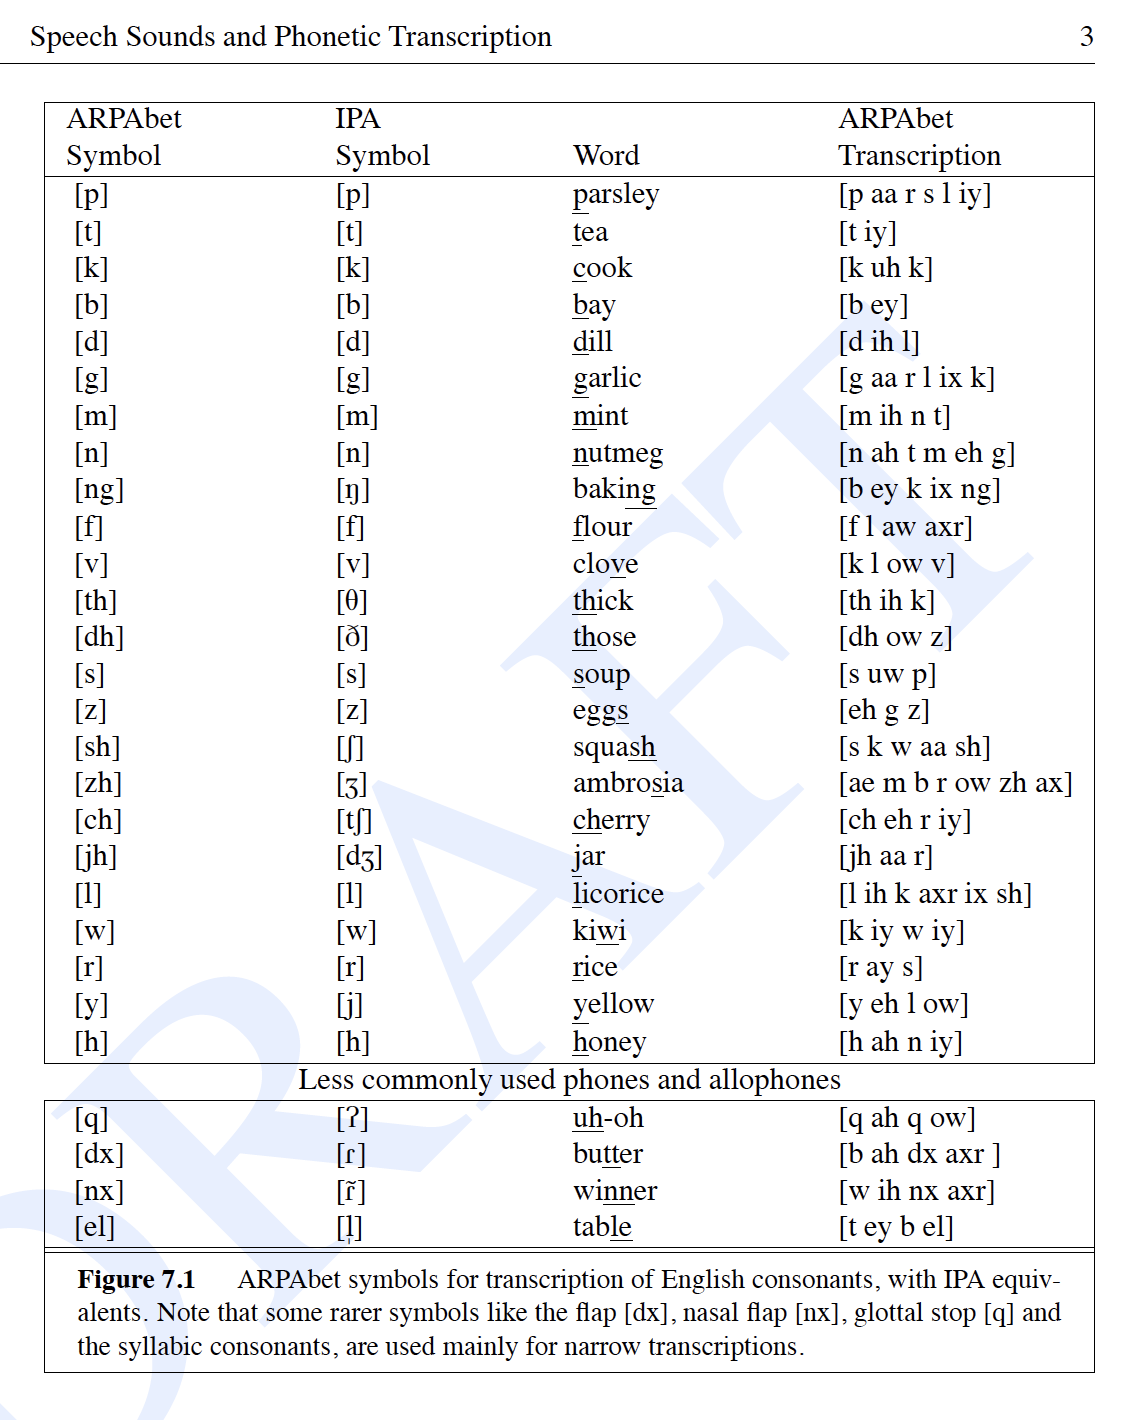
\includegraphics[width=0.6\textwidth]{arpabet.png}
\end{frame}

\begin{frame}
\frametitle{Alright, we know how to do transcription}
\begin{itemize}
\item So, let us say we prepare one exhaustive list of sounds in American English, or IPA or whatever we want.
\item We then build a pronunciation dictionary - where, unlike the traditional dictionary which gives you meaning of a word - this gives you how to pronounce that word.
\item So each time a user says something, let us say your program sees the spectrogram, and learns to cut the speech signal into individual sounds, stitch them into word sounds,  and then, you look up the dictionary to match sounds to real words. 
\item Does that sound alright so far? (I am obviously skipping details!) \pause
\item What else is missing after this point?
\end{itemize}
\end{frame}

\begin{frame}
\frametitle{Let me do a quick demo}
\begin{itemize}
\item Google Webspeech Demo. \url{https://www.google.com/intl/en/chrome/demos/speech.html}
\item (Notice how words change on screen - I have questions in the next slide!!!)
\item My text: "So now I'm trying to speak in Indian accent and we are going to see how good is the system with my accent"
\end{itemize}
\end{frame}

\begin{frame}
\frametitle{Questions on the demo}
\begin{itemize}
\item As I speak, you see words changing in the transcription sometimes after I moved on from that word and am speaking something else. Do you think it is just because the internet is slow or is there some other reason? \pause
\item What is the intuition behind choosing the words it is choosing? \pause
\item If I say the same thing twice, is it showing the same transcription? If it is different, why do you think it is different? \pause
\item Do you think we speak consistently in the same way, when we are speaking naturally? \pause
\item What causes speech variation between people? \pause
\item What causes speech variation between different versions of your own speech?
\end{itemize}
\end{frame}

\begin{frame}
\frametitle{Pronunciation Variation is Real - It is not only about non-native accents}
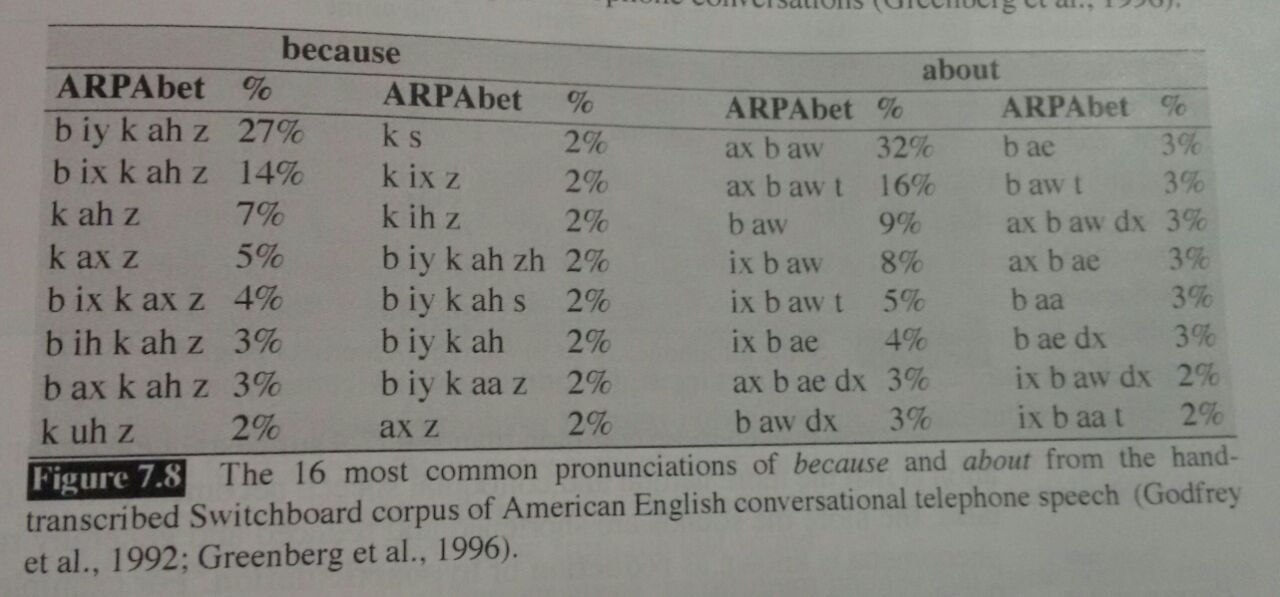
\includegraphics[width=0.9\textwidth]{because-about.jpeg}
\end{frame}

\begin{frame}
\frametitle{Why is there so much of variation?}
\framesubtitle{A short primer to our vocal tract}
\begin{itemize}
\item How is sound produced? - by rapid movement of air in the vocal organs of our body - from lungs through the trachea, and then out of mouth, and nose (nasal sounds)?
\item Consonants sounds can be distinguished:
\begin{itemize}
\item Depending on place of articulation (labial - lips coming together, dental, alveolar, palatal, velar, glottal)
\item Manner of articulation (nasal, voiced, unvoiced etc)
\end{itemize}
\item Similarly, different movements produce different vowels.
\item There can be stressed and unstressed sounds. 
\end{itemize}
Note: For more details, read on phonetics or talk to a linguist to get references.
\end{frame}

\begin{frame}
\frametitle{Factors influencing Phonetic Variation}
\begin{itemize}
\item Rate of speech (how fast does one speak)
\item Usage of different words - same letter can sound differently in context
\item Deletion of some part of the word while speaking
\item Gender, Social background, Dialect - all these influence your pronunciation
\item Over time, pronunciation of words change too!
\end{itemize}
Note: For more details, look for sociolinguistics videos or books. 
\end{frame}

\begin{frame}
\frametitle{Attendance Exercise}
\begin{itemize}
\item After all this discussion, what do you think are the different steps in speech recognition?
\item Also, here are four exchanges I had with Siri this morning: try to figure out what I meant and why it understood like this: 
\begin{itemize}
\item Me: Siri, I want to understand Holly work \\
Siri: Sorry, I couldn't find 'Holly' in your contacts.
\item Me: Siri, you really bad India next \\
Siri: But .... but.
\item Me: Can you recognize speech? \\
Siri: Do you want to increase or decrease the volume?
\item Me: No, can you do speech recognition? \\
Siri: Do you want to increase or decrease the volume?
\end{itemize}
\end{itemize}
\end{frame}

\end{document}

